	
	\section{Introduction}
	\label{section:intro}
    Acquiring knowledge from large volumes of unstructured textual data plays an important role in not only the development of Semantic
    Web, but also the understanding of text content. There has been an extensive body of work in transforming online encyclopedia resources, such as
    Wikipedia, into structured knowledge bases (\KBs) in a form of $\langle$\emph{subject entity},
   \emph{ predicate/relation}, \emph{object}$\rangle$ triples, such as DBpedia~\cite{Lehmann2009DBpedia,Auer2007DBpedia},
    Freebase~\cite{Bollacker2007Freebase}, Yago~\cite{Suchanek2008YAGO} etc.
    	

   %In order to better show the relations among entities,

	Such kind of \KBs can be naturally organized into the form of graphs which we call knowledge graphs (\KGs). Although most of those \KGs
originate from Wikipedia, they are usually created independently, thus often use different expressions and surface forms to indicate
equivalent entities and relations, let alone those built from different resources, or even different languages. This further makes it more
challenging to achieve knowledge sharing, complementary and integration among different \KGs.
	
	One of the key techniques to integrate different \KGs is \textbf{Entity Alignment}, the task of linking the equivalent entities from
different \KGs if they refer to the same real-world identity, usually with different surface forms. However, entity alignment is not a
trivial task, and the alignment system is often complex~\cite{gokhale2014corleone,scharffe2014ontology}. Traditional approaches, which
generally rely on external information such as hyperlinks in web pages and require costly manual feature construction, are often time
consuming and labor intensive~\cite{zhu2017iterative}.
	
	Most recently, many efforts have been devoted to the so-called KG embedding-based approaches, following similar ideas to jointly embed
the structures of multiple \KGs into a unified vector space with the pre-aligned entities or relations serving as a bridge. These
KG embedding-based approaches all rely on translation-based KG embedding models, such as TransE~\cite{bordes2013translating}, to learn
entity representations. However, as listed in Table~\ref{seed}, most of these KG embedding-based methods require high-quality seed
alignment data, such as pre-aligned KG predicates/relations or triples. Since the predicates/relations or triples in heterogeneous \KGs may
be very different, it is often difficult and expensive to collect such high-quality alignment data. In addition, as shown by the last
column in the Table~\ref{seed}, most of these models, except JAPE~\cite{sun2017cross}, ignore specific attribute values in the \KGs because
of their complexity and heterogeneity. And actually, JAPE only considers the types of those values for simplicity, and the specific
attribute values, such as \textit{1.86m} as someone's height, are ignored. However, values are actually very significant parts of \KGs, especially for low-quality \KGs which may contain large-scale values. The approaches that do not consider values will lose this part of information when aligning \KGs. We argue that those attribute value information are crucial for entity alignment and should be taken into account. 

\begin{table}
	\centering
	\scriptsize
	\begin{tabular}{l|llll}
		\toprule
		\bf Models & \bf entity & \bf relation & \bf triple & \bf use of value \\
		\midrule
		JE~\cite{hao2016joint} & ${\surd}$ & & & \\
		MTransE~\cite{chen2016multilingual} & $ $ & $ $ & ${\surd}$ & \\
		JAPE~\cite{sun2017cross} & ${\surd}$& ${\surd}$& & ${\surd}$ (type)\\
		ITransE~\cite{zhu2017iterative} & ${\surd}$ & ${\surd}$& & \\
		\bottomrule
	\end{tabular}
	\caption{The use of seed alignment information in each method.}
	\label{seed}
\end{table}
	
	Moreover, although TransE can effectively capture the structure information of \KGs, it may not perform well when the neighboring relational structures of two entities are significantly different. Since TransE utilizes the relation between the head entity and the tail entity to define the distance between the head entity vector and the tail entity vector, the TransE-based approaches actually tend to require that the neighboring structures of the equivalent entities from different \KGs should be as similar as possible. Nevertheless, due to the incompleteness of knowledge graphs, the densities of the neighborhoods of the two entities $e_1$ and $e_2$ that we need to align may be very different or similar relations and neighbors between $e_1$ and $e_2$ may be few, which leads to sparse available clues for alignment and will make a large difference between the learned vectors of $e_1$ and $e_2$ by TransE. But actually, when we judge whether two entities refer to the equivalent identity, we often only pay attention to the more informative and discriminative neighbors of the two entities, especially when the available clues are sparse.
	\begin{figure}
		\centering
			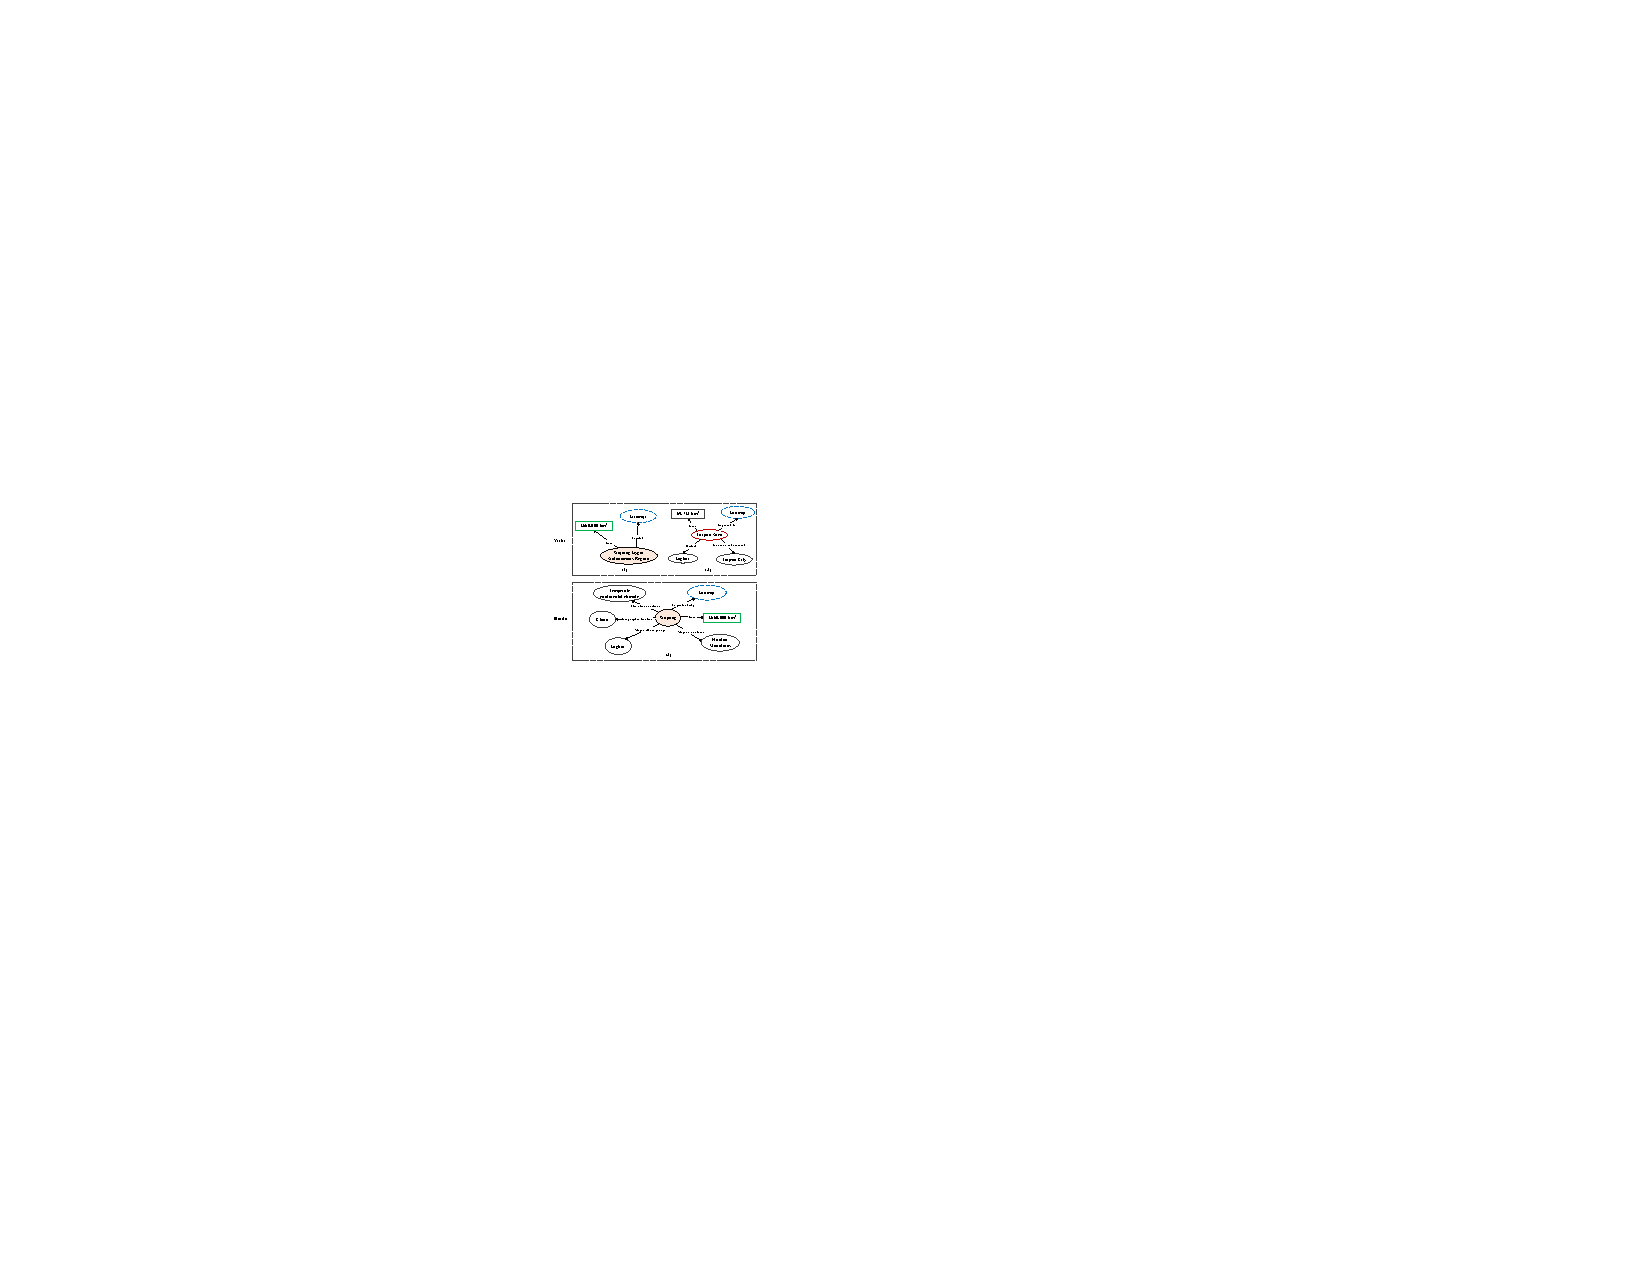
\includegraphics[width=1\linewidth]{figures/graph1.pdf}
			\caption{The neighborhoods of three entities extracted from Wiki and Baidu \KGs. The red circles indicate the aligned center entities. The blue circles represent the similar neighbors. The green rectangles indicate the same attribute values.}
			\label{Xinjiang}
	\end{figure}
	%The relational graph convolutional networks (R-GCNs), an extension of graph convolutional networks (GCNs) that operate on local graph neighborhoodsa recent class of multilayer neural networks operating on graphs, can better describe graph networks and facilitate the integration of semantic information into node features, which also makes it convenient to add value information. In addition, we believe that a favorable attention mechanism can further improve the ability to embed the nodes and can accurately extract structural information even in the absence of much information. By further introducing the attention mechanism, the graph attention networks(GATs) have been proposed. GAT computes the hidden representations of each node in the graph, by attending over its neighbors according to different weights, following a self-attention strategy.
	
	In this paper, we propose a new embedding-based entity alignment approach which leverages relational graph convolutional networks to better embed the highly multi-relational structure information of heterogeneous \KGs with a set of pre-aligned entities and considers the specific attribute values in multiple \KGs. Our model solves the limitations of existing embedding-based methods which ignore the value information and can not properly align the entities with very different neighborhoods.
	
	More specifically, the contributions of this paper can be summarized as follows:
	\begin{itemize}
		\item We propose RGCN, a novel entity alignment model, to better characterize entities in heterogeneous \KGs by considering their neighboring relational structure as well as the attribute values in the \KGs.
		
		\item We show that layer-wise highway gates play a significant role to control the balance of how much neighborhood information should be passed to a node in our HRGCN model.
		
		\item We build a large-scale entity alignment dataset in Chinese, containing 57,240 entities, 3,563 relations, 28,595 attributes, 231,003 relation triples and 515,065 attribute triples. We manually aligned 16,969 entity pairs as the gold standards of entity alignment.
		
	\end{itemize}
